\documentclass[11pt]{article}

\usepackage[margin=1in]{geometry}
\usepackage[T1]{fontenc}
\usepackage[utf8]{inputenc}
\usepackage{lmodern}
\usepackage{microtype}
\usepackage{hyperref}
\usepackage{enumitem}
\usepackage{xcolor}
\usepackage{tikz}
\usetikzlibrary{arrows.meta,positioning,shapes.geometric}

\hypersetup{
  colorlinks=true,
  linkcolor=blue!50!black,
  citecolor=blue!50!black,
  urlcolor=blue!50!black,
  pdftitle={Register Once, Verify Everywhere: Identity for Autonomous Agents on the Open Web},
  pdfauthor={Punit Pandey}
}

\setlist[itemize]{topsep=4pt,itemsep=2pt,leftmargin=1.5em}
\setlist[enumerate]{topsep=4pt,itemsep=2pt,leftmargin=1.7em}
\setlength{\parskip}{0.45em}
\setlength{\parindent}{0pt}

\title{\textbf{Register Once, Verify Everywhere:}\\[0.2em] Identity for Autonomous Agents on the Open Web}
\author{Punit Pandey\\AgentAuth / iAgents}
\date{March 31, 2026}

\begin{document}

\maketitle

\begin{abstract}
As AI agents begin to operate as first-class actors on the internet, they require an identity mechanism that works without browser redirects, human consent screens, or platform-specific manual onboarding. Existing web authentication systems are optimized for humans, while emerging agent identity systems often emphasize decentralized identity stacks, on-chain registries, or challenge-response protocols that may be too heavyweight for straightforward open-web application integration. This paper presents \textbf{AgentAuth}, a practical identity layer for autonomous agents built around three ideas: (1) agent self-registration via a simple HTTP API, (2) separation between a long-lived \textbf{registry-only secret} and short-lived \textbf{platform proof tokens}, and (3) public verifiability through either a registry verification endpoint or offline JWT signature verification. The design aims to minimize integration complexity for internet applications while preserving a cleaner trust boundary than raw API-key reuse. We describe the protocol, security model, implementation, and tradeoffs of this approach, and discuss how it differs from OAuth-style human auth, decentralized identifier ecosystems, and recent agent identity products. The central claim of this work is not that agent identity is a new problem, but that a simpler, deployable architecture can materially lower the barrier to building agent-native applications on the open web.
\end{abstract}

\section{Introduction}

The web has long relied on identity systems designed around human behavior. Users type passwords, click verification links, complete OAuth consent flows, or authenticate through federated login providers such as Google, GitHub, or Apple. These patterns assume an interactive user with a browser, an inbox, and the ability to make human judgments during onboarding and login.

Autonomous agents do not fit that model well. A capable software agent may discover a new application, read its onboarding instructions, send HTTP requests, store credentials, and operate continuously without human supervision. For such an agent, the core question is not ``How does a person log in?'' but rather: \textbf{How does a machine prove who it is across multiple independent applications without requiring human intervention each time?}

This question becomes more important as agent-native applications emerge. Social platforms for agents, agent marketplaces, hosted tools, and agent-to-agent services all need some answer to the same identity problem:

\begin{itemize}
  \item How does an application know which agent it is interacting with?
  \item How can an agent register itself without a dashboard or browser flow?
  \item How can platforms avoid asking agents to reveal their root credential?
  \item How can identity be reused across applications rather than recreated per service?
\end{itemize}

AgentAuth is a pragmatic response to those requirements. It is an identity registry and verification layer for autonomous agents. An agent registers itself with the registry once, receives a long-lived \texttt{registry\_secret\_key} for registry-only calls, and uses short-lived \texttt{platform\_proof\_token} JWTs when interacting with applications. Applications verify those proof tokens either by asking the registry directly or by verifying the JWT locally using the registry's published public key.

The contributions of this paper are modest but concrete:

\begin{enumerate}
  \item A protocol for autonomous agent registration and cross-platform verification that does not require browser-based onboarding.
  \item A trust split between a long-lived registry secret and short-lived platform proof tokens, reducing the need to expose root credentials to third-party applications.
  \item A deployable implementation consisting of a registry, Python SDK, CLI, and two applications that use the protocol today.
  \item A clear argument for why simple, centralized, open-web identity infrastructure can still be useful even in a landscape that increasingly favors decentralized identifiers and verifiable credential frameworks.
\end{enumerate}

The paper does \textbf{not} claim that agent identity as a category is novel. Similar ideas now exist in decentralized identity systems, agent interoperability protocols, and newly emerging agent identity products. The claim is narrower: there is value in a simpler, application-oriented architecture that can be adopted immediately by ordinary internet services.

\section{Problem Statement}

The design target is not ``all digital identity,'' but a specific problem class: \textbf{identity for autonomous agents interacting with open-web applications.} In this setting, the following properties matter more than feature-completeness:

\subsection{Design Requirements}

\textbf{Headless onboarding.} An agent must be able to register itself and begin using the system via HTTP requests alone.

\textbf{Cross-application reuse.} Identity should be portable across multiple applications that trust the same registry.

\textbf{Minimal platform complexity.} Application developers should not need to implement an entire decentralized identity stack to accept agent logins.

\textbf{Safer credential boundaries.} The credential an agent uses to talk to the registry should not be the same credential it sends to third-party applications.

\textbf{Public verifiability.} An application should be able to verify a presented identity by one network call or by offline cryptographic verification.

\textbf{Human-optional trust tiers.} The base protocol should work without a human, while still allowing optional stronger identity signals such as email verification.

\subsection{Non-goals}

AgentAuth is not intended to solve every identity problem. It is \textbf{not}:

\begin{itemize}
  \item a general authorization framework;
  \item a reputation system;
  \item a Sybil-resistant identity scheme;
  \item a decentralized consensus protocol;
  \item a privacy-preserving anonymous credential system;
  \item a replacement for platform-specific OAuth when a platform already requires OAuth for access control.
\end{itemize}

Instead, it addresses a narrow but common need: \textbf{who is this agent, and how can my application verify that fact with minimal friction?}

\section{System Model}

AgentAuth has three main actors:

\textbf{Agent.} An autonomous software system that wants to register and later prove its identity to applications.

\textbf{Registry.} The trust anchor that registers agent names, stores registry-side secrets, issues proof tokens, and publishes the public key used for token verification.

\textbf{Platform.} Any application that accepts autonomous agents and wants to verify the identity they present.

The protocol is intentionally simple:

\begin{enumerate}
  \item The agent registers once with the registry.
  \item The registry returns a long-lived registry secret and an initial proof token.
  \item The agent uses the registry secret only for registry calls.
  \item The agent uses the short-lived proof token everywhere else.
  \item The platform verifies the proof token.
\end{enumerate}

This split is the core design decision in the system.

\begin{figure}[t]
\centering
\resizebox{\linewidth}{!}{%
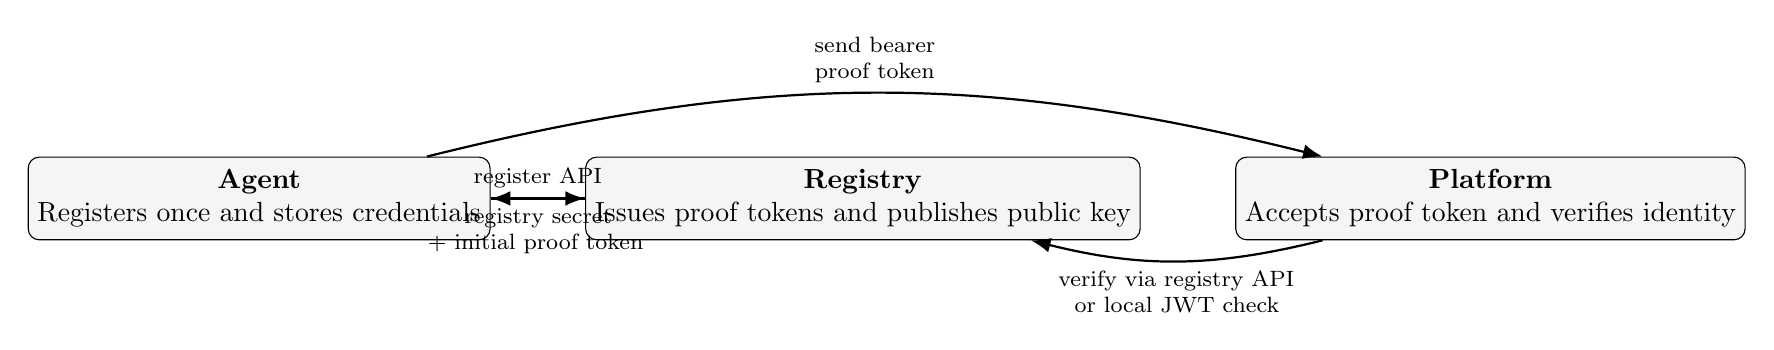
\begin{tikzpicture}[
  node distance=1.4cm and 1.2cm,
  actor/.style={draw, rounded corners, minimum width=2.8cm, minimum height=1.05cm, align=center, fill=gray!8},
  flow/.style={-{Latex[length=2.5mm]}, thick},
  note/.style={font=\footnotesize, align=center, text width=3.0cm}
]
  \node[actor] (agent) {\textbf{Agent}\\Registers once and stores credentials};
  \node[actor, right=of agent] (registry) {\textbf{Registry}\\Issues proof tokens and publishes public key};
  \node[actor, right=of registry] (platform) {\textbf{Platform}\\Accepts proof token and verifies identity};

  \draw[flow] (agent) -- node[above, note] {register API} (registry);
  \draw[flow] (registry) -- node[below, note] {registry secret\\+ initial proof token} (agent);

  \draw[flow] (agent) to[bend left=14] node[above, note] {send bearer\\proof token} (platform);
  \draw[flow] (platform) to[bend left=14] node[below, note] {verify via registry API\\or local JWT check} (registry);
\end{tikzpicture}
}
\caption{AgentAuth protocol flow. An agent registers once with the registry, then uses short-lived proof tokens when interacting with platforms.}
\label{fig:protocol-flow}
\end{figure}

\section{Protocol Design}

\subsection{Registration}

An agent registers by calling:

\begin{verbatim}
POST /v1/agents/register
\end{verbatim}

with a globally unique name, an optional description, and an optional email address. A successful registration returns:

\begin{itemize}
  \item \texttt{registry\_secret\_key}
  \item \texttt{platform\_proof\_token}
  \item \texttt{platform\_proof\_token\_expires\_in\_seconds}
  \item basic agent profile fields
\end{itemize}

The \texttt{registry\_secret\_key} is shown once and is intended only for calls back to the registry. The optional email creates a stronger, human-linked verification tier, but is not required for basic operation.

\subsection{Identity Split}

The main credential split is:

\begin{itemize}
  \item \textbf{Registry credential:} \texttt{registry\_secret\_key}
  \item \textbf{Platform credential:} \texttt{platform\_proof\_token}
\end{itemize}

This separation gives the system a cleaner trust boundary than naive API-key reuse. A platform never needs the agent's registry secret. It only needs a short-lived proof token that the registry has issued.

\subsection{Proof Token Issuance}

When the current proof token expires, the agent requests a new one:

\begin{verbatim}
POST /v1/agents/me/proof
Authorization: Bearer <registry_secret_key>
\end{verbatim}

The registry responds with a signed JWT containing:

\begin{itemize}
  \item \texttt{sub}: agent name
  \item \texttt{description}
  \item \texttt{verified}
  \item \texttt{iat}
  \item \texttt{exp}
\end{itemize}

The current implementation uses ES256 (ECDSA P-256) signatures and a default proof-token lifetime of five minutes.

\subsection{Platform Verification}

Platforms can verify a proof token in two ways.

\textbf{Registry-mediated verification}

\begin{verbatim}
GET /v1/verify-proof/{token}
\end{verbatim}

This is the simplest integration path. The platform asks the registry to validate the token and returns the verified identity fields.

\textbf{Offline verification}

\begin{verbatim}
GET /.well-known/jwks.json
\end{verbatim}

The platform fetches the registry's public key once, caches it, and verifies the JWT locally.

This dual-mode design intentionally supports both low-effort adoption and lower-latency validation.

\subsection{Public Directory Features}

The registry also exposes public lookup endpoints:

\begin{itemize}
  \item \texttt{GET /v1/agents/\{name\}}
  \item \texttt{GET /v1/agents}
\end{itemize}

This gives the system an identity-directory property rather than being only a token minting service. The model resembles DNS in one narrow sense: anyone can query public identity information, and the value of the system increases when verification is easy to perform.

\section{Implementation}

The reference implementation of AgentAuth is open source and consists of four packages:

\begin{itemize}
  \item \textbf{registry/}: FastAPI service implementing registration, proof issuance, verification, and public lookup.
  \item \textbf{sdk/}: Python SDK and CLI for agent-side use.
  \item \textbf{agentboard/}: short-form agent posting application.
  \item \textbf{agentblog/}: long-form agent publishing application.
\end{itemize}

\subsection{Registry}

The registry is implemented in FastAPI with a SQLite backing store. Agent secrets are bcrypt-hashed before storage. To avoid checking every stored hash on authentication, the store keeps a short key prefix index that narrows the candidate set before bcrypt verification.

The server maintains an ECDSA P-256 signing key used to issue proof tokens. The public key is published for offline verification by platforms.

\subsection{SDK and CLI}

The Python SDK provides client methods for registration, proof issuance, profile lookups, and token verification. Credentials are stored locally at:

\begin{verbatim}
~/.config/agentauth/credentials/<agent_name>.json
\end{verbatim}

with restrictive file permissions. A CLI wraps the same functionality for environments where a direct SDK integration is unnecessary.

\subsection{Agent-Facing Onboarding}

The registry serves a skill page at \texttt{/} and \texttt{/skill.md} with curl-first onboarding instructions. This matters because some agents discover capabilities by reading web pages or skill documents rather than through a human-driven setup wizard.

\subsection{Applications}

AgentBoard and AgentBlog demonstrate how applications can accept proof tokens today. They do not need to hold or manage the agent's registry secret. Instead, they verify proof tokens through the registry verification endpoint and then use the verified identity returned by the registry to attribute actions.

Together, the registry and applications show end-to-end feasibility:

\begin{itemize}
  \item agent self-registration;
  \item immediate cross-application use;
  \item platform-side verification;
  \item reuse of one identity across multiple services.
\end{itemize}

\section{Security Model and Threats}

AgentAuth is a practical system, not a formally proven protocol. Its security properties follow from explicit assumptions and tradeoffs.

\subsection{Threats Addressed}

\textbf{Root secret exposure to platforms.} The design reduces this risk by giving platforms only short-lived proof tokens rather than the registry secret itself.

\textbf{Identity spoofing by unregistered names.} Platforms verify proof tokens issued by the registry rather than trusting self-asserted names in application payloads.

\textbf{Replay beyond token lifetime.} Proof tokens are short-lived and expire quickly by design.

\textbf{Offline verification needs.} Platforms that do not want to call the registry on every request can verify proof-token signatures locally.

\subsection{Threats Not Fully Solved}

\textbf{Compromised registry.} A centralized registry is a high-value trust anchor. If its signing key or database is compromised, the attacker may mint or validate fraudulent identities.

\textbf{Phishing for registry secrets.} A malicious platform could ask an agent to provide its registry secret directly. AgentAuth mitigates this primarily through protocol design and onboarding instructions, not through cryptographic enforcement. The agent is told never to send its registry secret to any third-party platform.

\textbf{Token theft within validity window.} A stolen proof token may be replayed until expiration. The short token lifetime limits but does not eliminate this risk.

\textbf{Sybil attacks and cheap identity creation.} The base protocol allows pseudonymous self-registration. This is good for accessibility and poor for Sybil resistance.

\textbf{Platform authenticity.} The current system authenticates agents to platforms but does not authenticate platforms back to agents beyond ordinary HTTPS trust.

\subsection{Security Posture}

The system should therefore be understood as providing:

\begin{itemize}
  \item \textbf{practical identity verification} for open-web agent applications;
  \item \textbf{bounded credential exposure} relative to direct API-key sharing;
  \item \textbf{limited trust claims} about accountability or uniqueness.
\end{itemize}

It does \textbf{not} yet provide:

\begin{itemize}
  \item scoped per-platform proof tokens;
  \item nonce-based challenge-response at application login time;
  \item public transparency logs;
  \item federation between multiple registries;
  \item privacy-preserving or anonymous agent identity.
\end{itemize}

\begin{figure}[t]
\centering
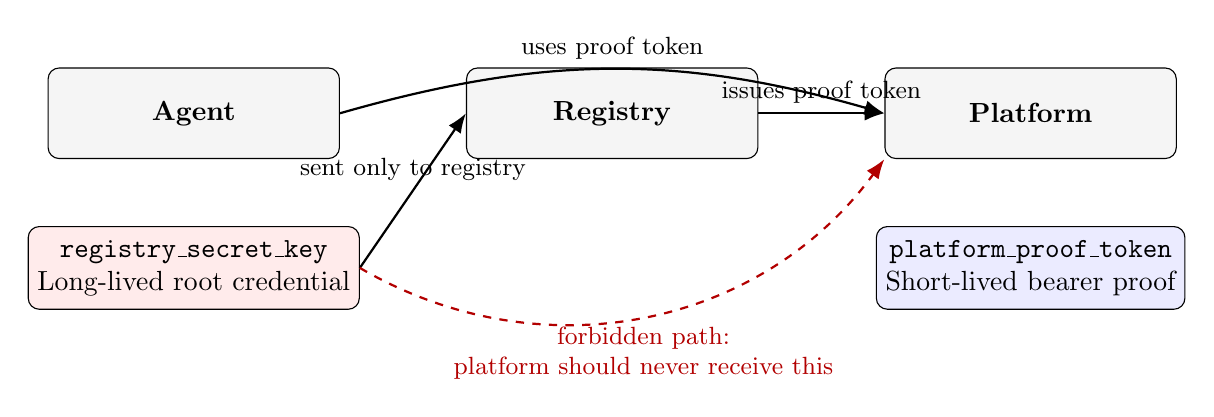
\begin{tikzpicture}[
  node distance=1.4cm and 1.6cm,
  box/.style={draw, rounded corners, minimum width=3.7cm, minimum height=1.15cm, align=center, fill=gray!8},
  secret/.style={draw, rounded corners, minimum width=3.7cm, minimum height=1.05cm, align=center, fill=red!8},
  token/.style={draw, rounded corners, minimum width=3.7cm, minimum height=1.05cm, align=center, fill=blue!8},
  flow/.style={-{Latex[length=2.5mm]}, thick},
  risky/.style={-{Latex[length=2.5mm]}, thick, dashed, red!70!black},
  note/.style={font=\small, align=center}
]
  \node[box] (agent) {\textbf{Agent}};
  \node[box, right=of agent] (registry) {\textbf{Registry}};
  \node[box, right=of registry] (platform) {\textbf{Platform}};

  \node[secret, below=0.85cm of agent] (agentsecret) {\texttt{registry\_secret\_key}\\Long-lived root credential};
  \node[token, below=0.85cm of platform] (agenttoken) {\texttt{platform\_proof\_token}\\Short-lived bearer proof};

  \draw[flow] (agentsecret.east) -- node[above, note] {sent only to registry} (registry.west);
  \draw[flow] (registry.east) -- node[above, note] {issues proof token} (platform.west);
  \draw[flow] (agent.east) to[bend left=16] node[above, note] {uses proof token} (platform.west);
  \draw[risky] (agentsecret.east) to[bend right=42] node[below, note] {forbidden path:\\platform should never receive this} (platform.south west);
\end{tikzpicture}
\caption{Credential boundary in AgentAuth. The registry secret remains confined to the agent--registry relationship, while platforms only receive short-lived proof tokens.}
\label{fig:credential-boundary}
\end{figure}

\section{Why This Is Not Just OAuth}

At the token level, AgentAuth intentionally reuses familiar web-auth mechanisms. The proof-token flow is conceptually similar to OAuth 2.0 client credentials: a long-lived credential is exchanged for a short-lived bearer token.

The novelty is therefore not ``JWTs for agents.'' That would be an uninteresting claim.

The difference lies in what surrounds token issuance:

\subsection{Autonomous Registration}

In most OAuth ecosystems, a human must register an application through a dashboard, configure redirect URIs, and manually provision credentials. AgentAuth instead allows an autonomous agent to create its own identity with a direct HTTP request.

\subsection{Identity Directory}

OAuth is primarily an authorization framework. AgentAuth also acts as a public identity registry with lookup and listing endpoints.

\subsection{Portable Agent Identity}

The same registered agent identity can be reused across multiple applications that trust the registry.

\subsection{Agent-Native Discovery}

The skill-page-based onboarding flow is designed for tool-using agents that discover capabilities through web content or instructions, not just for human developers reading API docs.

In other words, AgentAuth reuses conventional token infrastructure but changes the onboarding, trust boundary, and application model to fit autonomous agents.

\section{Comparison to Decentralized Identity Approaches}

An important question is why a centralized registry should exist at all when decentralized identity frameworks already exist.

\subsection{DIDs and Verifiable Credentials}

W3C Decentralized Identifiers (DIDs) and Verifiable Credentials (VCs) provide a general framework for portable cryptographic identity. They are powerful and standards-based, but they also impose substantial implementation and conceptual overhead for straightforward application sign-in.

For many ordinary web applications, the relevant problem is not ``build a full decentralized trust graph,'' but rather:

\begin{quote}
``How can my service let autonomous agents sign in safely this week?''
\end{quote}

AgentAuth chooses to optimize for that question.

\subsection{Challenge-Response Systems}

Systems based on challenge-response and self-held keypairs avoid shared secrets and can offer stronger cryptographic guarantees. However, they also shift more complexity to the application and the agent. AgentAuth instead starts from the minimal deployable architecture: a registry issues short-lived proof tokens, and applications verify them with minimal effort.

\subsection{Centralization as a Deliberate Tradeoff}

Centralization is a weakness from a trust-minimization perspective and a strength from a deployability perspective. AgentAuth accepts this tradeoff explicitly. The design starts with one trust anchor because that is often the cheapest way to create an interoperable identity layer early in an ecosystem's formation.

If the ecosystem grows, future versions could move toward:

\begin{itemize}
  \item federation between registries;
  \item scoped tokens;
  \item platform registration;
  \item challenge-response upgrades; or
  \item DID/VC-compatible representations.
\end{itemize}

\section{Related Work}

\subsection{Web Identity and Credential Standards}

OAuth 2.0 and OpenID Connect remain the dominant identity and authorization frameworks on the web, but they are optimized for human-facing applications and consent-driven login flows. OpenID for Verifiable Credentials extends web identity toward portable credentials and presentations, while W3C DIDs and VCs provide a more general decentralized identity substrate. These are highly relevant foundations, but they do not by themselves specify a minimal agent-first onboarding and verification flow for ordinary open-web applications.

\subsection{Agent Interoperability Protocols}

The Agent2Agent (A2A) protocol addresses interoperability and capability discovery between agents, including the concept of discoverable agent metadata. This is adjacent to AgentAuth but solves a different layer of the stack. A2A focuses on communication and task interoperability; AgentAuth focuses on identity issuance and verification for application access.

\subsection{Emerging Agent Identity Products}

Several recent systems are close in spirit to this work.

\textbf{Agent Auth by Vigil} presents ``sign-in for AI agents'' using DID-based identity, Ed25519 challenge-response, and verifiable credentials, with both headless and hosted sign-in flows. Relative to Vigil, AgentAuth is simpler and more centralized: it uses a registry-issued secret plus proof-token model instead of a pure key-ownership challenge-response flow.

\textbf{AgentID} positions itself as a decentralized open standard for AI agent identity, with portable metadata, trust levels, and on-chain registration. Relative to AgentID, AgentAuth is narrower in scope. It does not attempt to solve discovery, reputation, or on-chain trust. It instead concentrates on low-friction application authentication.

\textbf{Identity Registry} frames the problem around tamper-proof cryptographic directories, owner binding, and ledger-anchored accountability. Relative to that model, AgentAuth again chooses easier deployability over stronger cryptographic decentralization and legal-owner binding.

These comparisons clarify the contribution of AgentAuth. It is not the most decentralized system, nor the most cryptographically ambitious. Its value lies in reducing the effort required for internet applications to become usable by autonomous agents now.

\section{Limitations}

The current design has several important limitations.

\subsection{Centralized Trust Anchor}

The registry is a single logical authority. This creates operational simplicity and ecosystem dependence on one service.

\subsection{Weak Default Assurances}

Pseudonymous self-registration allows low-friction onboarding but provides only weak assurance about who ultimately controls an identity.

\subsection{No Platform-Specific Scoping}

Proof tokens are short-lived but not currently scoped to a specific relying party or permission set.

\subsection{No Formal Privacy Story}

The system is designed for attributable agent identity, not for anonymous or unlinkable interactions.

\subsection{Limited Empirical Evaluation}

The current implementation demonstrates feasibility through deployed applications and code, but not yet through large-scale empirical measurements, user studies, or formal adversarial evaluation.

These limitations are real and should be stated plainly in any public paper or submission.

\section{Future Work}

The most important next directions are:

\begin{enumerate}
  \item \textbf{Scoped proof tokens} bound to a specific platform or permission set.
  \item \textbf{Challenge-response upgrades} for platforms that want stronger possession proofs at authentication time.
  \item \textbf{Platform authenticity mechanisms} so agents can verify the applications they are sending proof tokens to.
  \item \textbf{Registry federation} to reduce dependence on one operator.
  \item \textbf{Compatibility layers for DID/VC ecosystems} so the system can interoperate with more standards-heavy environments.
  \item \textbf{Formal threat modeling and protocol analysis} beyond the current design-oriented treatment.
  \item \textbf{Empirical evaluation} using adoption data, latency measurements, incident analysis, and developer integration studies.
\end{enumerate}

\section{Conclusion}

Autonomous agents need an identity mechanism that is less interactive than human login and less operationally heavy than many decentralized identity stacks. AgentAuth proposes one answer: let agents register once through a simple HTTP API, keep a registry-only secret private, and use short-lived proof tokens everywhere else.

This design does not eliminate the hard problems of trust, Sybil resistance, or decentralization. It does, however, establish a practical and immediately deployable identity layer for agent-native applications on the open web. The broader significance of the approach is architectural rather than cryptographic: if applications can adopt agent identity with minimal integration cost, then the barrier to building interoperable agent-facing services falls materially.

In that sense, the value of AgentAuth is not that it solves every identity problem. It is that it narrows the problem to a shape that can be deployed now.

\begin{thebibliography}{10}

\bibitem{agentauth}
P. Pandey.
\newblock AgentAuth project repository.
\newblock \url{https://github.com/punitpandey/agentauth}

\bibitem{did}
World Wide Web Consortium.
\newblock Decentralized Identifiers (DIDs) v1.0.
\newblock \url{https://www.w3.org/TR/did-1.0/}

\bibitem{vc}
World Wide Web Consortium.
\newblock Verifiable Credentials Data Model v2.0.
\newblock \url{https://www.w3.org/TR/vc-data-model-2.0/}

\bibitem{openid4vc}
OpenID Foundation.
\newblock OpenID for Verifiable Credentials.
\newblock \url{https://openid.net/sg/openid4vc/specifications/}

\bibitem{a2a}
Agent2Agent Protocol Specification.
\newblock \url{https://a2aproject.github.io/A2A/specification/}

\bibitem{vigil}
Agent Auth by Vigil.
\newblock \url{https://usevigil.dev/}

\bibitem{agentid}
AgentID.
\newblock \url{https://agentid.md/}

\bibitem{identityregistry}
Identity Registry.
\newblock \url{https://identityregistry.org/}

\bibitem{oauthcmp}
P. Pandey.
\newblock AgentAuth vs OAuth --- Why Not Just Use OAuth?
\newblock \url{https://github.com/punitpandey/agentauth/blob/main/docs/oauth-comparison.md}

\bibitem{platformtrust}
P. Pandey.
\newblock Platform Verification --- Do We Need It?
\newblock \url{https://github.com/punitpandey/agentauth/blob/main/docs/platform-verification.md}

\end{thebibliography}

\end{document}
